\chapter{ЭКСПЕРИМЕНТЫ И ОЦЕНКА РЕЗУЛЬТАТОВ РАБОТЫ}

В данной главе рассматривается этап оценки работы подсистемы
управления движением. Описанные проведенные эксперименты по проверке
работы системы управления

\section{Экспериментальное исследование подсистемы движения по траектории }
Подсистема движения по траектории играет важную роль в работе системы управления движением автомобиля, т.к. точное
следование траектории требуется, чтобы автомобиль двигался так, как было запланировано системой планирования движения,
чтобы обеспечить безопасное и оптимальное движение.

Были произведены испытания подсистемы движения по траектории отдельно от системы планирования движения.
На вход системы подавались искусственно сформированные траектории различной формы, осуществлялось движение модели
автомобиля по этой траектории, и оценивалось реальная траектория с помощью визуального наблюдения, измерения расстояния
между ключевыми точками траектории и анализируя траекторию движения, полученную с ZED-камеры. На рисунке
\ref{img:path_moving_test}. По результатам испытаний было установлено, что максимальное отклонение при движении
по окружности радиус 1.5 м составило 50 мм.

\begin{figure}[h]
    \centering
    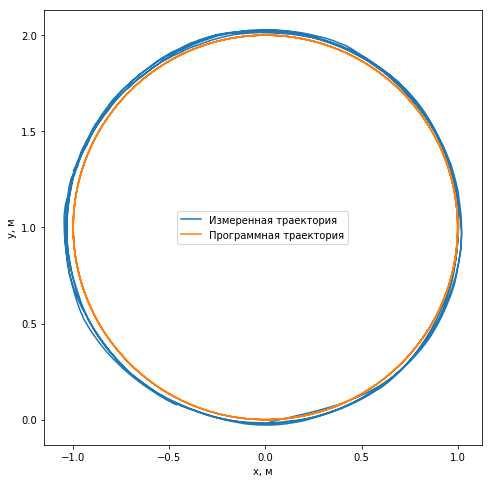
\includegraphics[width=0.7\linewidth]{images/path_moving_test}
    \caption{Результаты эксперимента с движением по заданной траектории}
    \label{img:path_moving_test}
\end{figure}

\section{Экспериментальное исследование подсистемы планирования локального движения}

Подсистема планирования локального движения является одной из ключевых подсистем в системе управления беспилотным
автомобилем. Был произведен ряд экспериментов с использованием мобильной колесной платформы для оценки работы алгоритмов.

Первый вариант подсистемы планирования движения основывался на алгоритме A, планируя геометрический путь в обход
препятствия, когда оно пересекало опорную траекторию.
Алгоритм был реализован и испытан на мобильной платформе. По результатам испытаний были выявлены дополнительные
недостатки алгоритма. В связи с неидеальностью системы компьютерного зрения, при обновлении периодическом Occupancy Grid
происходит небольшое "мерцание", т.е. те или иные пограничные ячейки карты могут менять свое состояние. Это приводит
к тому, что алгоритм резко перестраивает траекторию движения. Особенно это было заметно, когда модель приближалась
к симметричному препятствию. В таком случае, алгоритм мог прокладывать обходную траекторию то по левую сторону от
препятствия, то по правую сторону от препятствия. Это приводило к тому, что модель не могла корректно осуществить
маневр и врезалась в препятствие.

По результатам испытаний было выявлено, что рассмотренный алгоритм не подходит для локального планирования траекторий
движения беспилотного автомобиля.

Следующий вариант подсистемы планирования движения движения использует планирование траектории в форме полиномов пятого
порядка и учитывает текущую ориентацию и скорость модели, чтобы планировать движения по гладким траекториям.
Результаты испытаний этого алгоритма показали, что алгоритм способен осуществлять движение по опорной траектории,
осуществляя маневры для объезда препятствий с последующим возвратом на траекторию. Результат работы алгоритма
приведен на рисунке \ref{img:obstacle_avoidance}.

\begin{figure}[h]
    \centering
    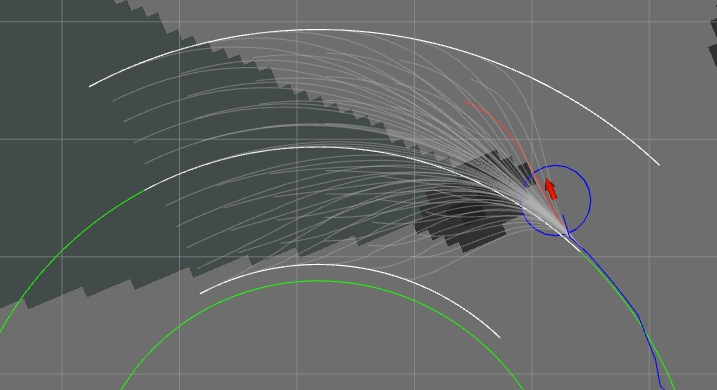
\includegraphics[width=\linewidth]{images/obstacle_avoidance}
    \caption{Результаты эксперимента с движением по заданной траектории}
    \label{img:obstacle_avoidance}
\end{figure}

На этом рисунке изображено движение автомобиля, обозначенного
красной стрелкой, по опорной траектории (зеленая линия) в форме спирали. Толстые белые линии обозначают границу области
планирования поперечных траекторий. Набор белых линий представляет траектории-кандидаты, сгенерированные алгоритмом
планирования движения, а красная линия ~--- выбранную оптимальную траекторию.

\section{Выводы по главе}

Было проведено экспериментальное исследование работы различных подсистем системы управления движением
беспилотного автомобиля (системы обнаружения препятствий, системы движения по траектории, системы планирования локального
движения) как по отдельности, так и совместно в составе системы управления движением. Полученные результаты
свидетельствуют о работоспособности разработанных алгоритмов.